
Necesitaremos una plataforma donde desplegar el programa de control que disponga de las características necesarias para interactuar con el hardware del  motor de corriente continua y la electrónica de potencia: el puente H. Las soluciones más comerciales son arduino y raspberry.
Vamos a poner a prueba la versatilidad de Golang para compilar el programa en distintas arquitecturas de chips de CPU de forma trasparente para el programador.
Se elige Raspberry como plataforma para albergar el código cliente por poseer una interfaz más amigable de cara al desarrollo y las pruebas del programa.
Se entiende que el ámbito del proyecto ya es lo suficientemente complejo y arduino pudiera requerir mayor de esfuerzo debido a no disponer de sistema operativo a la hora de trabajar.

En la~\cref{fig:raspberry pins} se puede ver los pines disponibles para acceder desde el sistema operativo y en la~\cref{fig:Used Pins} hemos señalado los que va a utilizar nuestro diseño.

\begin{figure}[H]
    \centering
    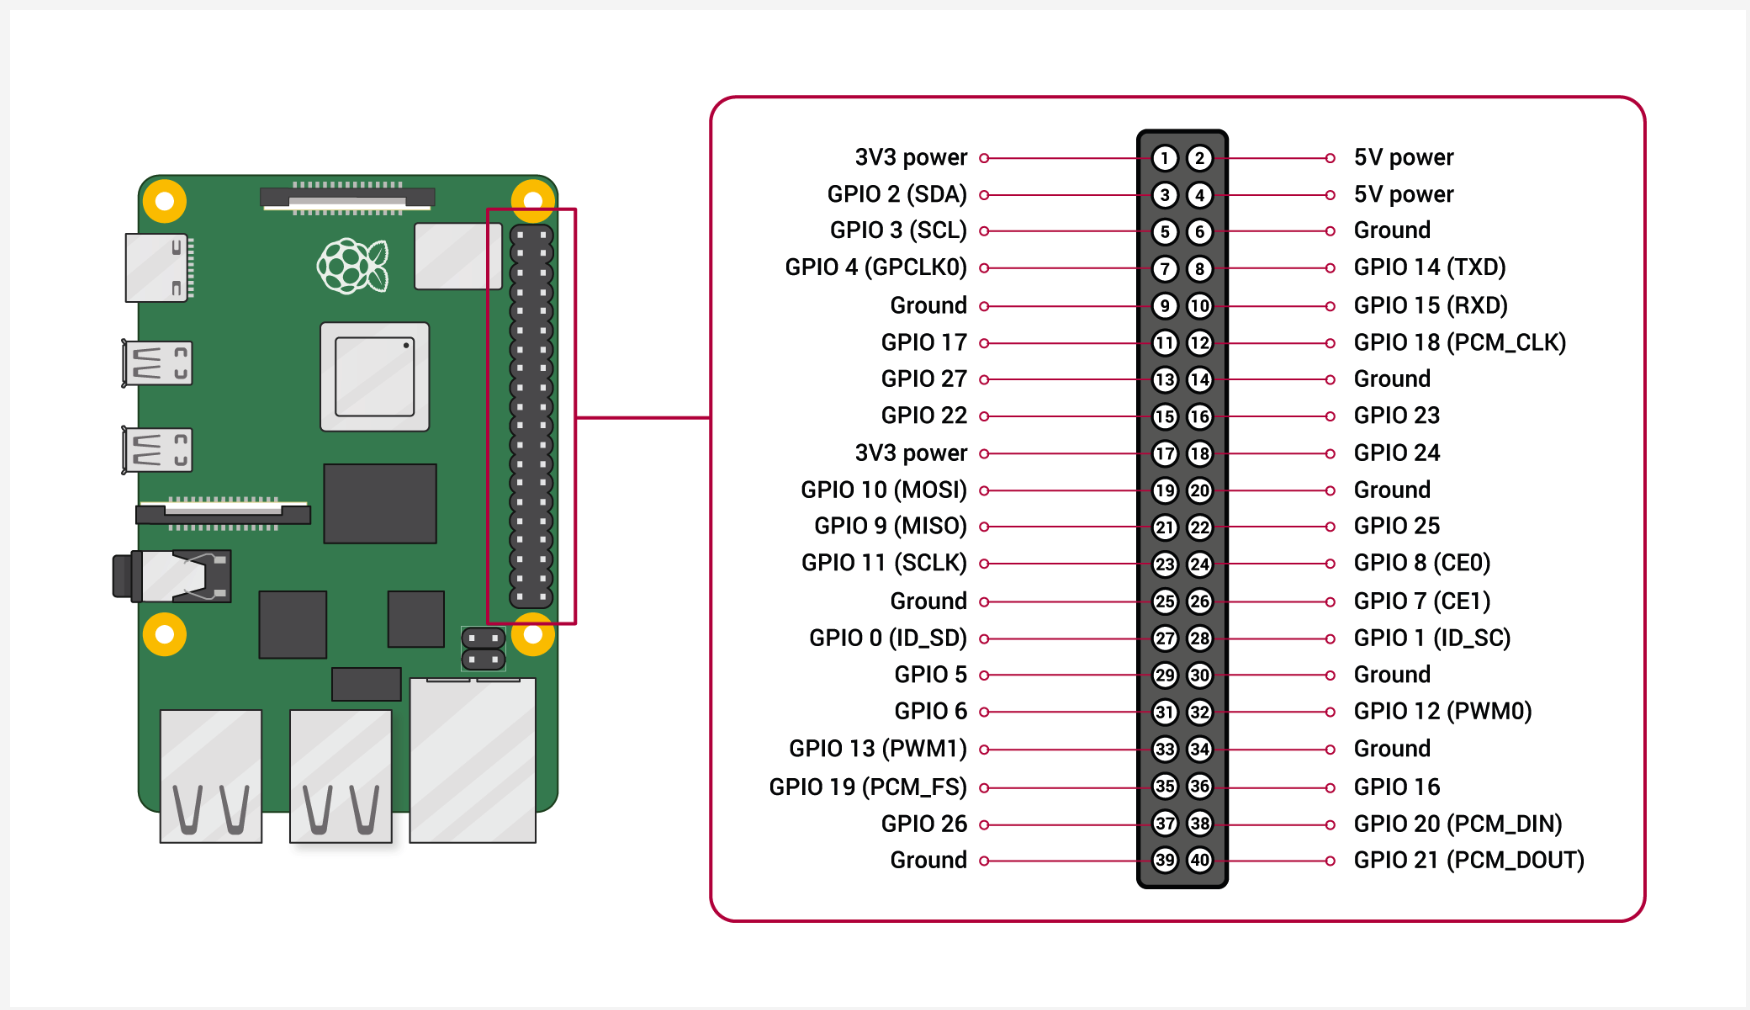
\includegraphics[scale = 0.4]{part/Proyecto_ejecutivo/memoria_constructiva/raspb/img/raspberry}
    \caption{PinSet de Raspberry Pi 4.4\cite{raspberryORG} }\label{fig:raspberry pins}
\end{figure}

\begin{figure}[H]
    \centering
    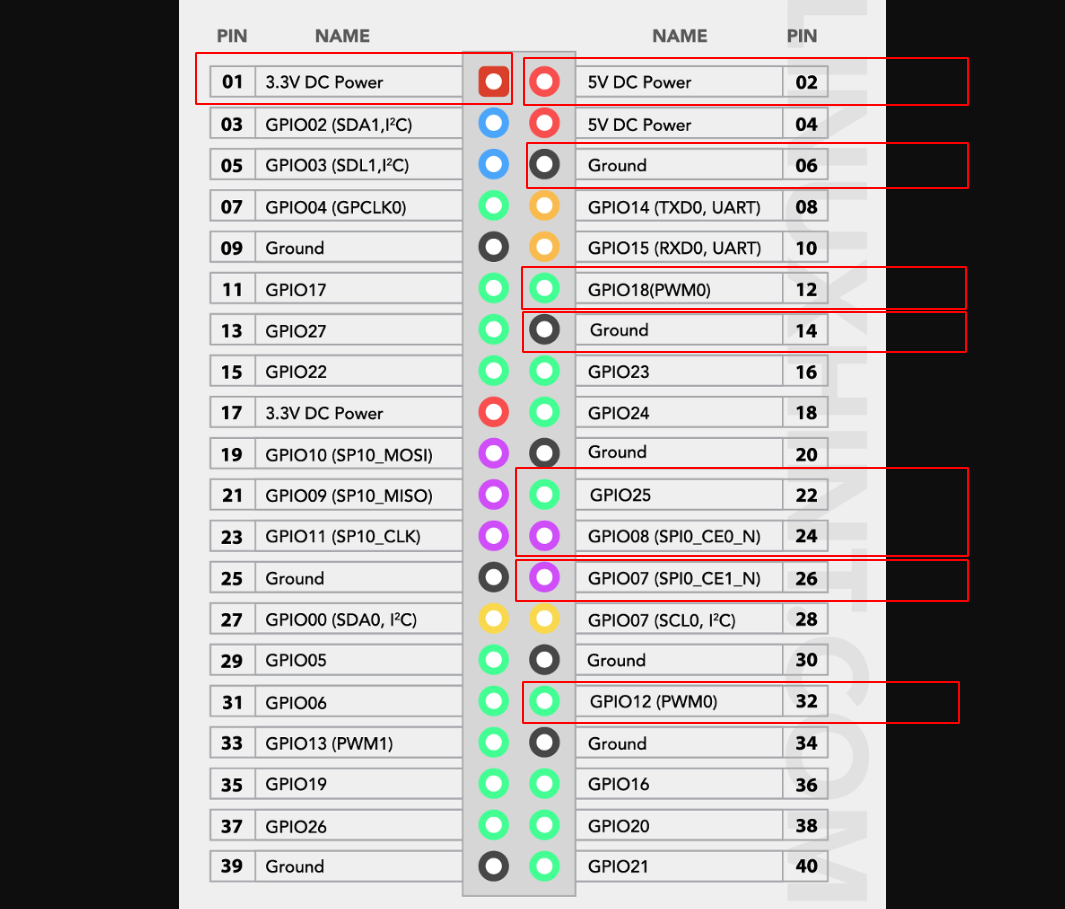
\includegraphics[scale = 0.4]{part/Proyecto_ejecutivo/memoria_constructiva/raspb/img/gpio-pinout-raspberry-pi-01-used}
    \caption{Pins utilizados en el proyecto}\label{fig:Used Pins}
\end{figure}